\documentclass{beamer}
\setbeamercovered{transparent}
\usepackage{listings}
\usepackage[T1]{fontenc}

\usetheme[pageofpages=of,% String used between the current page and the
                         % total page count.
          bullet=circle,% Use circles instead of squares for bullets.
          titleline=true,% Show a line below the frame title.
          titlepagelogo=opensuse,
          alternativetitlepage=true,% Use the fancy title page.
          ]{Torino}


% Define some stiles
\lstdefinestyle{mybash}{
  language=bash,
  basicstyle=\footnotesize\ttfamily,
  keywordstyle=\color{blue}\ttfamily,
  stringstyle=\color{red}\ttfamily,
  commentstyle=\color{green}\ttfamily,
  morecomment=[l][\color{magenta}]{\#}
}

\lstdefinestyle{myperl}{
  language=Perl,
  basicstyle=\footnotesize\ttfamily,
  keywordstyle=\color{blue}\ttfamily,
  stringstyle=\color{red}\ttfamily,
  commentstyle=\color{green}\ttfamily,
  morecomment=[l][\color{magenta}]{\#}
}


\setbeamerfont{title}{series=\bfseries,size=\LARGE}
\author{Alberto Planas,\newline Ludwig Nussel\newline {\tiny SUSE Linux Products GmbH}}
\title{openQA Workshop -- oSC14}
\subtitle{Learning how to make tests with openQA}


\AtBeginSection[]{
  \setbeamercolor{background canvas}{bg=chameleongreen3}
  \begin{frame}[plain]
    \begin{center}\begin{huge}\textcolor{white}{\secname}\end{huge}\end{center}
  \end{frame}
  \setbeamercolor{background canvas}{bg=}
}

\AtBeginSubsection[]{
  \setbeamercolor{background canvas}{bg=chameleongreen3}
  \begin{frame}[plain]
    \begin{center}\begin{huge}\textcolor{white}{\subsecname}\end{huge}\end{center}
  \end{frame}
  \setbeamercolor{background canvas}{bg=}
}


\begin{document}

\begin{frame}[t,plain]
  \titlepage
\end{frame}


\section{Introduction}
%
% Architecture
%
\begin{frame}{Architecture}
  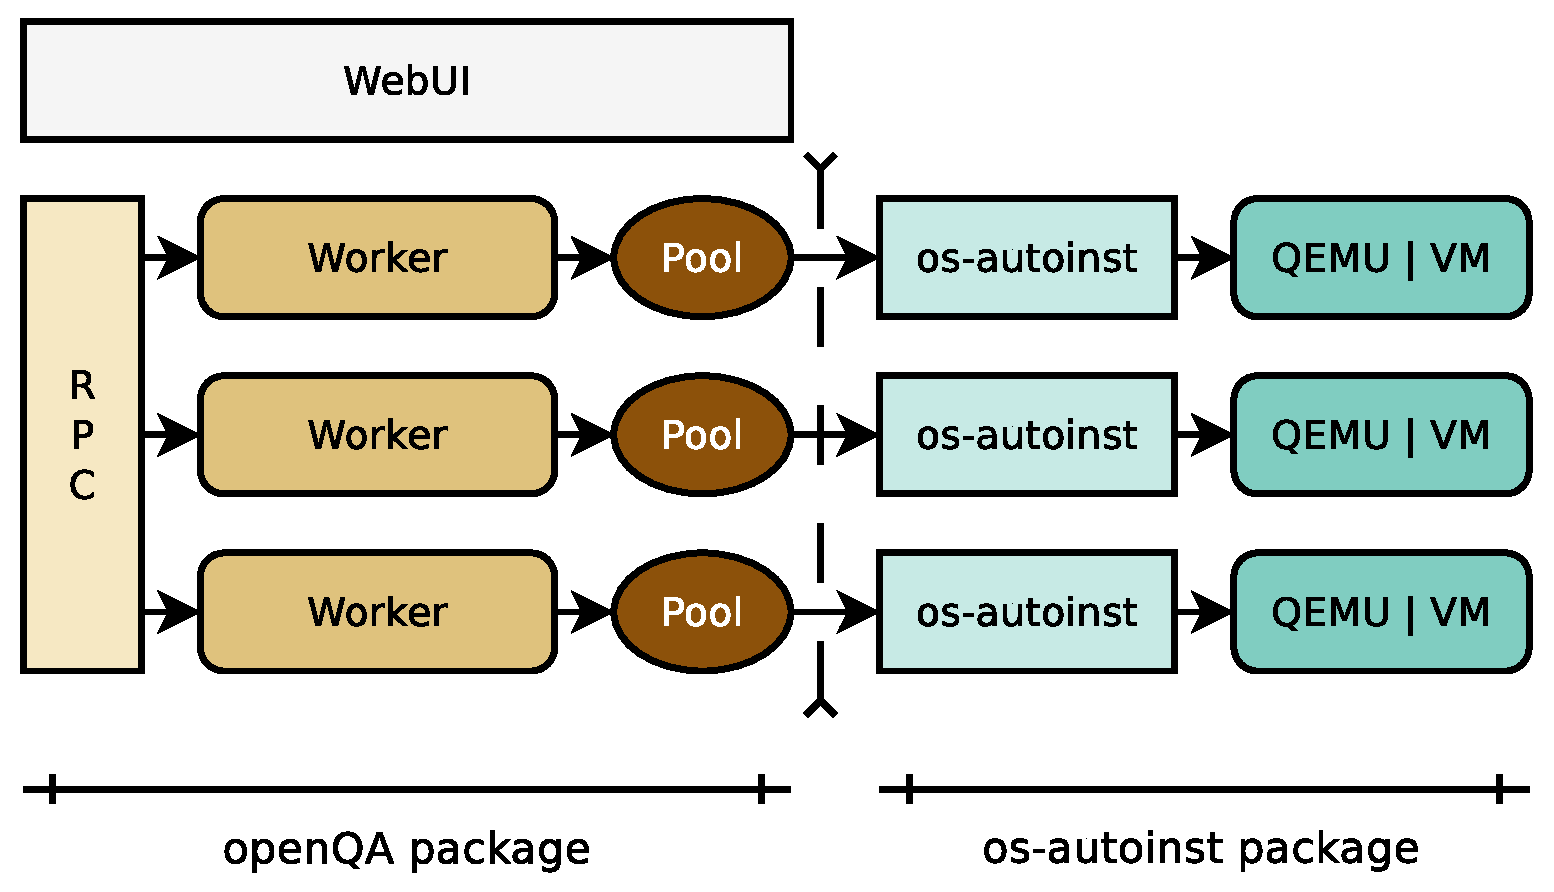
\includegraphics[height=5.8cm,width=10.3cm]{arch}
\end{frame}

%
% Overview
%
\begin{frame}{Overview}
  In this workshop we will ...
  \begin{itemize}
    \item start with testing a small live distro
    \item learn how to create or modify reference images
    \item learn how to create tests
  \end{itemize}
\end{frame}

\section{Installation}
%
% Installation
%
%\begin{frame}[fragile]
%  \frametitle{Installation}
%  TODO: add ancor's slide
%\end{frame}

%
% Installation
%
\begin{frame}[fragile]
  \frametitle{Installation}
  \begin{itemize}
  \item install packages
    \lstset{style=mybash}
    \begin{lstlisting}
zypper ar -f obs://devel:openQA/openSUSE_13.1 openQA
zypper ar -f obs://devel:openQA:13.1/openSUSE_13.1 \
  openQA-perl-modules
zypper in openQA apache2
    \end{lstlisting}
    \item start web interface
    \begin{lstlisting}
systemctl start openqa-webui
    \end{lstlisting}
  \item More detailed instructions at \newline
    \url{https://github.com/os-autoinst/openQA}
  \end{itemize}
\end{frame}

\begin{frame}[fragile]
  \frametitle{Apache Setup}
  \begin{itemize}
    \item use default vhost template
    \lstset{style=mybash}
    \begin{lstlisting}
cp /etc/apache2/vhosts.d/openqa.conf.template \
   /etc/apache2/vhosts.d/openqa.conf
    \end{lstlisting}
\item enable required apache modules
    \begin{lstlisting}
a2enmod headers
a2enmod proxy
a2enmod proxy_http
    \end{lstlisting}
    \item (re)start apache
    \begin{lstlisting}
rcapache2 restart
    \end{lstlisting}
  \end{itemize}
\end{frame}

\begin{frame}[fragile]
  \frametitle{Generate Secrets for Authentication}
  \begin{itemize}
    \item switch off https in \texttt{/etc/openqa/openqa.ini}
    \begin{lstlisting}
[openid]
httpsonly = 0
    \end{lstlisting}
    \item go to \url{http://localhost/} and log in
    \item go to Admin -> Secrets and generate a pair of key+secret
    \item edit \texttt{/etc/openqa/client.conf} and put key and secret there
  \end{itemize}
\end{frame}

% opensuse specific, we have dsl as example later though
%\begin{frame}[fragile]
%  \frametitle{fetch tests and reference images}
%  \begin{itemize}
%    \item the \texttt{fetchneedles} tool gets openSUSE data from github
%    \lstset{style=mybash}
%    \begin{lstlisting}
%/usr/lib/os-autoinst/tools/fetchneedles
%    \end{lstlisting}
%  \end{itemize}
%\end{frame}


%\begin{frame}{Screenshot}
%  \includegraphics[height=6.2cm,width=10.88cm]{screenshot}
%\end{frame}
%

\section{openQA Usage}
%
% Running a Test
%
\begin{frame}[fragile]
  \frametitle{Pick some small distro to practice with}
  \begin{itemize}
  \item download SliTaz
    \lstset{style=mybash}
    \begin{lstlisting}
wget -P /var/lib/openqa/factory/iso \
  http://mirror.slitaz.org/iso/4.0/ \
  slitaz-4.0.iso
    \end{lstlisting}
  \item clone template repo for distro
    \lstset{style=mybash}
    \begin{lstlisting}
cd /var/lib/os-autoinst/tests
sudo -u geekotest \
  git clone git://github.com/os-autoinst/ \
  os-autoinst-distri-example.git slitaz
ln -s /var/lib/os-autoinst/tests/slitaz \
  /usr/lib/os-autoinst/distri/
    \end{lstlisting}
  \end{itemize}
\end{frame}

%
% Exercise 1
%
\begin{frame}[fragile]{Exercise 1 -- Testing an ISO}
  \begin{enumerate}
  \item Create a job for the ISO
    \lstset{style=mybash}
    \begin{lstlisting}
/usr/share/openqa/script/client jobs post \
  DISTRI=slitaz VERSION=4.0 ARCH=i586 \
  TEST=foo MACHINE=bar NICMODEL=e1000 \
  DESKTOP=default ISO=slitaz-4.0.iso
    \end{lstlisting}
  \item Launch one worker
    \lstset{style=mybash}
    \begin{lstlisting}
systemctl start openqa-worker@1.service
    \end{lstlisting}
  \item Watch in the web UI live until it fails!
  \end{enumerate}
\end{frame}

%
% Test Failed
%
\begin{frame}{Test Failed}
  So... the test failed. Let's see what happened.
  \begin{itemize}
  \item Go to the result view
  \item Click on the thumbnail of the failed test
  \item Check the screenshot
  \item Check the "Source code" tab to see the test code
  \end{itemize}
\end{frame}

%
% The Needle
%
\begin{frame}[fragile]
  \frametitle{The Needle}
  A needle is a PNG image and a metadata in JSON
  \begin{columns}
    \begin{column}{0.45\textwidth}
    \lstset{style=mybash}
    \begin{lstlisting}
      {
        "area": [
          {
            "width": 514,
            "xpos": 255,
            "type": "match",
            "ypos": 0,
            "height": 538
          }
        ],
        "tags": [
          "inst-instmode"
        ]
      }
    \end{lstlisting}
    \end{column}

    \begin{column}{0.45\textwidth}
      \includegraphics[height=4cm,width=5.33cm]{needle}
    \end{column}
  \end{columns}
\end{frame}

%
% Exercise 2
%
\begin{frame}{Exercise 2 -- Create a Needle}
  \begin{enumerate}
  \item Restart the test and open the new job
  \item Set the job to interactive mode
  \item Stop the test when it's at the bootloader
  \item Create a needle in the failing test
  \item Be careful with the Tags!
  \end{enumerate}
\end{frame}


\section{openQA API}
%
% Exercise 3
%
\begin{frame}{Exercise 3 -- Modify a Test}
  \begin{enumerate}
  \item Tests are in \texttt{/var/lib/os-autoinst/tests}
  \item Find the slitaz ones and have a look at the directories
  \begin{itemize}
    \item Test driver: \texttt{main.pm}
    \item Actual tests: \texttt{test.d}
    \item Needles: \texttt{needles}
  \end{itemize}
  \item Open the boot test, figure out what is doing and modify it
  \end{enumerate}
\end{frame}

\begin{frame}[fragile]{Modified Test}
    \begin{lstlisting}
+    waitforneedle( "language", 30 );
+    sendkey "ret";
+
+    waitforneedle( "keyboard", 30 );
+    sendkey "ret";
+
+    waitforneedle( "keyboard_text", 30 );
+    sendkey "ret";
    \end{lstlisting}
\end{frame}


%
% API
%
%
% Anatomy of a test
%
\begin{frame}[fragile]
  \frametitle{Anatomy of a Test I}
    \lstset{style=myperl}
    \begin{lstlisting}
      use base "basetest";
      use strict;
      use bmwqemu;

      # Determine, using the $ENV variables, if the
      # test can be selected for this configuration.
      sub is_applicable() {
      }

      # Main code of the test
      sub run() {
      }
    \end{lstlisting}
\end{frame}


\begin{frame}{Variables}
  Typcial variables available in openSUSE
  \begin{itemize}
  \item DESKTOP = kde | gnome | lxde | minimalx ...
  \item DISTRI | VERSION | ARCH | TEST | MACHINE
  \item USBBOOT | LIVETEST | NETBOOT
  \item BTRFS | ENCRYPT | LVM | RAIDLEVEL
  \item UEFI
  \end{itemize}
\end{frame}

\begin{frame}{API for Input}
  Sending events to the VM
  \begin{itemize}
  \item \texttt{sendkey "alt-n";} -- Send a keystroke
  \item \texttt{sendkey \$cmd\{"next"\};} -- Use the \texttt{\$cmd\{\}} map for shortcuts
  \item \texttt{sendautotype "string";} -- Send a set of keys
  \item \texttt{sendautotype("string", 3);}
  \end{itemize}
\end{frame}

\begin{frame}{API for Needles}
  Sending events to the VM
  \begin{itemize}
  \item \texttt{waitforneedle("tag", 1);} -- Assert needle with this tag
  \item \texttt{checkneedle("tag", 1);} -- Return needle if needle found
  \item \texttt{\$self->check\_screen;} -- Assert using a synthetic tag name (\texttt{test-\$testname-\$count})
  \item \texttt{\$self->take\_screenshot;} -- Do not assert. Journal for the test
  \end{itemize}
\end{frame}

\begin{frame}[fragile]
  \frametitle{Anatomy of a Test II}
    \lstset{style=myperl}
    \begin{lstlisting}
      # Return a map of flags to decide if the fail
      # of this test is important, or to decide a
      # rollback of the VM status.
      sub test_flags() {
      }

      1;
    \end{lstlisting}
\end{frame}

\begin{frame}{Test Flags}
  With the tests flags we control the behavior of the test if it fails.
  \begin{itemize}
  \item \texttt{\{ 'fatal'=>1 \}} -- If fails, the test suite stops in failed state
  \item \texttt{\{ 'important'=>1 \}} -- If fails, the overall state fails. ISO considered broken
  \item \texttt{\{ 'milestone'=>1 \}} -- If ok, generate a new 'lastgood' snapshot
  \item \texttt{\{ \}} -- If fails, recover the 'lastgood' snapshot and continue to the next test
  \end{itemize}
\end{frame}


%
% Exercise 4
%
\begin{frame}{Exercise 4 -- A test for nano}
  Problem: SliTaz has not default keyboard bindings
  \begin{enumerate}
  \item Create a test for nano
  \item switch to text console
  \item log in as root (password root)
  \item launch nano
  \item exit it again
  \end{enumerate}
\end{frame}


\begin{frame}[fragile]
  \frametitle{The test for nano}
  \lstset{style=myperl}
  \begin{lstlisting}
sub run {
    sendkey "ctrl-alt-f1";
    waitforneedle( "console", 30 );
    sendautotype "root\n";
    sendautotype "root\n";
    sendautotype "nano\n";
    waitforneedle( "nano", 30 );
}
  \end{lstlisting}
\end{frame}

%\begin{frame}[fragile]
%  \frametitle{A test for Okular -- Sleeping}
%  But is not working!! -- We need to sleep.
%  \lstset{style=myperl}
%  \begin{lstlisting}
%    [...]
%    sub run() {
%      my $self=shift;
%      sendkey "alt-f2"; sleep 2;
%      sendautotype "okular"; sleep 2;
%      sendkey "ret"; sleep 2;
%      waitforneedle("okular", 5);
%      sendkey "alt-f4"; sleep 2;
%      sendkey "ret";
%    }
%    [...]
%  \end{lstlisting}
%\end{frame}

\begin{frame}{API to Run Programs}
  We can hide the sleep command... a bit.
  \begin{itemize}
  \item \texttt{script\_run("program");} -- Run the program from a terminal
  \item \texttt{script\_sudo("program");} -- Run the program as root
  \item \texttt{x11\_start\_program("program");} -- You have implemented that
  \end{itemize}
\end{frame}

%
% Exercise 5
%
\begin{frame}{Exercise 5 -- install a package}
  \begin{enumerate}
    \item install the sudo package (\texttt{tazpkg get-install sudo})
    \item exit the shell
    \item log in as tux (no password)
  \end{enumerate}
\end{frame}


%
% Exercise 5
%
\begin{frame}{Exercise 5 -- The sudo Case}
  \begin{enumerate}
  \item From time to time we want to run a program with sudo
  \item sudo sometimes asks but not always
  \item Figure out how to resolve this problem with the current API
  \item If you are out of ideas, find the implementation and try to understand it
  \end{enumerate}
\end{frame}


\begin{frame}[fragile]
  \frametitle{The sudo Case}
  Solution: checkneedle
  \lstset{style=myperl}
  \begin{lstlisting}
    sendautotype("sudo ls\n");
    if (checkneedle("sudo-prompt", 2)) {
      sendautotype("p4ssw0rd");
      sendkey "ret";
    }
  \end{lstlisting}
\end{frame}

\begin{frame}[fragile]
  \frametitle{A Complex Case}
  How to resolve when a dialog box appears during the installation process?
  \lstset{style=myperl}
  \begin{lstlisting}
    my @tags = (@{needle::tags("good-needle")},
                @{needle::tags("bad-needle")});
    my $err = 0;
    while (1) {
      my $ret = waitforneedle(\@tags, 200);
      last if $ret->{needle}->has_tag("good-needle");
      $self->take_screenshot;
      sendkey "ret";
      $err = 1;
    }
    mydie if $err;
  \end{lstlisting}
\end{frame}


\begin{frame}{Advanced API}
  \begin{itemize}
  \item \texttt{qemusend "command";} -- Send QEMU commands directly
  \item \texttt{makesnapshot "name";} -- Create a VM snapshot
  \item \texttt{loadsnapshot "name";} -- Recover a VM snapshot
  \item \texttt{mouse\_[move|set|click](x, y);} -- Control the mouse
  \item \texttt{mouse\_hide;} -- Hide the mouse
  \item \texttt{waitserial "regexp";} -- Result 1 if found in the serial port
  \end{itemize}
\end{frame}


\section{Questions?}

\begin{frame}{Suse is hiring}
  \begin{figure}
    \includegraphics[width= 0.8\linewidth]{suse_hiring.png}
  \end{figure}
\end{frame}

\begin{frame}{Thanks}
  \begin{center}
    Thank you for your attention.
  \end{center}
\end{frame}

\end{document}

% vim: et sw=2
